\documentclass[12pt]{article}
\usepackage{mathtools,amssymb}
\usepackage{enumitem}
\usepackage{multicol,tikz}
\usepackage{fullpage}

\title{Beginner Test 3}
\author{Stellenbosch Camp 2024}
\date{$3$ hours}

\begin{document} \maketitle

Note that the below problems are \emph{not} arranged in order of difficulty.

\begin{enumerate}[topsep=2\bigskipamount,itemsep=\bigskipamount]

%%%% Yves
\item On my digital clock the time is {\bf 02:46}.
In how many minutes will the four digits $0$, $2$, $4$ and $6$, in any order, next appear? 

\item In the sum $ab + ba = ca6$, different letters represent different digits.
Determine the value of $a+b+c$.

\item Find the last digit of the number $17^{100}$.

\item Determine the remainder when $38^{24}+39^{77}$ is divided by $7$ .


%%%% Muphulusi
\item If $a+b = 1$ and $a^2+b^2 = 2$, what is the value of $a^5+b^5$?

\item Solve for the positive real number $x$ if $x>1$ and $x^{x^4} = 64$.

\item Factorise $x^4 +4$. (Hint: add and subtract $4x^2$.)


%%%% Naeem
\item How many different natural numbers $n$ are there such that $n^{2}-440$ is a perfect square?

\item The largest integer $n$ for which $n^{200} < 5^{300}$ is?

\item Let $f$ be a function such that for all real numbers $x$,
\[ f(x+1) = x^{2}+5x+3. \]
What is $f(x-1)$?


%%%% Liam
\item How many integers between $1$ and $1200$ are \emph{not} a multiple of $3$, of $4$, or of $5$?

\pagebreak
\item
\begin{multicols}{2}
    Antony the Ant starts at a point $P$ in an infinite grid as in the figure.
    At each move, he can move one unit either to the left, to the right, upwards, or downwards, and after $20$ moves he wants to end up back where he started at point $P$.
    How many different paths can he take to do so where the number of horizontal moves is the same as the number of vertical moves?

    \begin{center} 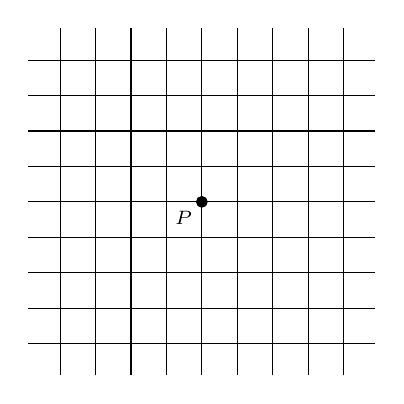
\begin{tikzpicture}[scale=0.45]
        \tikzstyle{every node} = [font=\scriptsize]
        \draw[step=1] (-4.9,-4.9) grid (4.9,4.9);
        \filldraw (0,0) circle[radius=0.15] node[below left] {$P$};
    \end{tikzpicture} \end{center}
\end{multicols}

\item Muphulusi had a bag with infinitely many red, green, blue, black, and white stones.
He grabbed $10$ stones out of the bag, and noticed that there were no red stones among the stones he grabbed.
Or maybe there were no green stones; he can't remember.
How many different possible groups of $10$ stones could he have grabbed?

%%%% Kate

\item
\begin{multicols}{2}
Six circles, each with radius 2, have been arranged in the shape below. Some of the circles are shaded white, and some grey. Some areas in between the circles have also been shaded grey. What is the area of the shaded region?

Hint 1: Consider drawing all the circles out.\\
Hint 2: Consider how you may break up the shapes in between circles and move those pieces around.

\centering
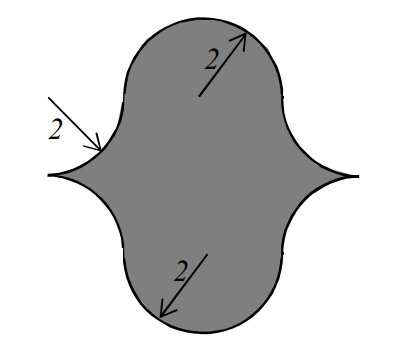
\includegraphics[width=0.4\textwidth]{sem.png}
\end{multicols}

\item
\begin{multicols}{2}
We know exactly two things about this shape:
\begin{itemize}
    \item [1.] All sides ($AB$, $BC$, $CE$, $DE$, $AD$, $AE$, $BE$) are integers.
    \item [2.] $CE = 9$ units.
\end{itemize}
Show why $CE$ cannot be $7$ units long.

Hint: Prove by contradiction.    

\centering
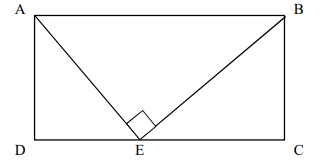
\includegraphics[width=\linewidth]{pythagtriples.png}
\end{multicols}

\pagebreak
\item
\begin{multicols}{2}
This diagram shows two squares, A and B, inside a larger square.
Find the ratio of the area of A to the area of B. 

\centering
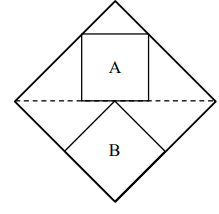
\includegraphics[width=0.8\linewidth]{trisquare.png}
\end{multicols}

\item
\begin{multicols}{2}
The grid below is made up of $1cm \times 1cm$ squares. All vertices (corners) of the shaded shape lie on the corners of squares. What is the area of the shaded shape?

\centering
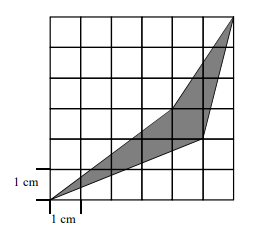
\includegraphics[width=0.8\linewidth]{boomerang.png}
\end{multicols}

\end{enumerate}

\end{document}